\section{太赫兹无线通信的主要挑战}
很明显,最近在电子和光子太赫兹收发器设计方面的进展已经实现了高效的信号生成、调制和辐射。经过审查的大多数太赫兹无线通信系统都低于300 GHz,为了达到大于1Tbps的数据速率,工作频率将高于300~500GHz。根据国际半导体技术路线图(International Technology Roadmap for Semiconductors, ITRS),硅互补金属氧化物半导体(Si-CMOS)的截至频率将在几年内超过500 GHz。但在实际应用中仍面临诸多挑战。以下是太赫兹无线通信面临的主要挑战。

\subsection{传播损耗与功率}

太赫兹波段的电磁波在空气中极易被水蒸气、氧气等分子吸收,导致信号衰减严重。水蒸气对太赫兹波的吸收尤为显著,尤其是在高湿度环境下,信号衰减会进一步加剧。这种吸收效应限制了太赫兹通信的传输距离,通常仅适用于短距离通信场景。目前基于电子的太赫兹系统产生的功率通常低于
10 mW。因此,除非采用高增益天线,否则传输距离非常
短。随着功率和工作频率的提高,功耗和散热可能成为主
要问题,因为导电材料的欧姆损耗与频率成正比,而太赫
兹设备和系统的尺寸必然很小。

\subsection{精密电子器件的制造}

虽然射频/微波设备的制造已经成熟,但太赫兹设备的制造还不成熟。基本的二极管和晶体管在太赫兹波段还不能很好地工作。高精度的机械加工已经生产出许多高质量的毫米波和亚太赫兹天线和波导,但难以满足更高频率的要求。当半导体器件的工作频率高达太赫兹频段,半导体材料的影响和器件封装的分布式参数效应直接影响电路和系统的性能。

到目前为止,2DEG复合材料
(如GaN HEMT)和2D材料(如石墨烯)\cite{10698344}已经被应用于太赫兹调制器。因此,未来可以开发在太赫兹波段响应时
间小于1 ps的人造材料,用于器件的制造。

\begin{figure}[htbp]
	\centering
	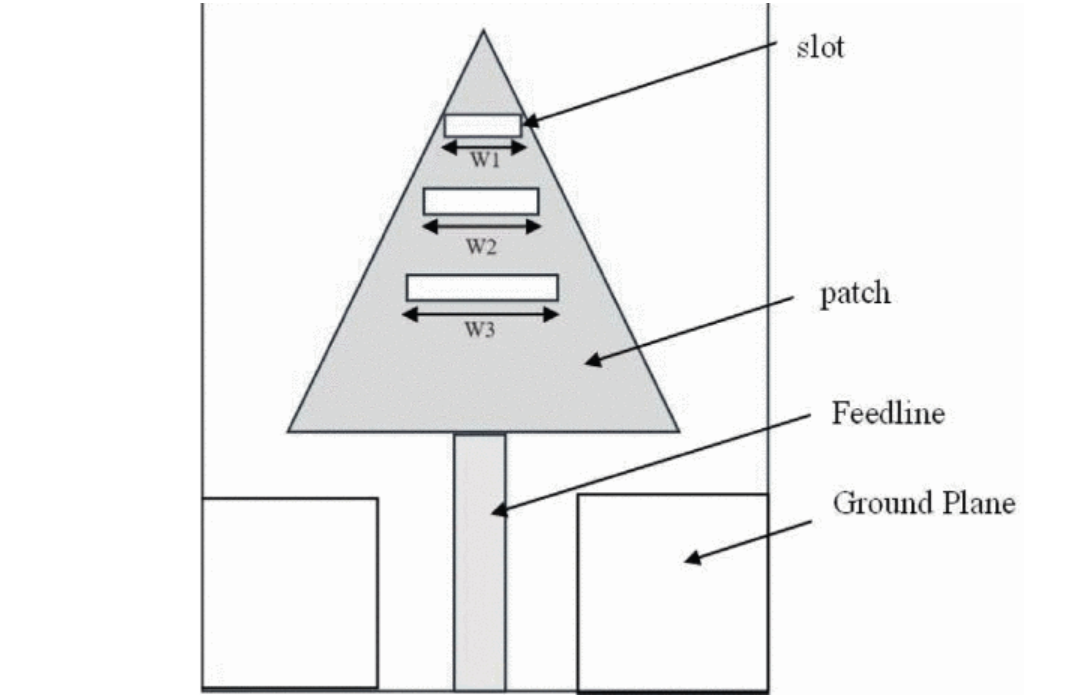
\includegraphics[width=0.6\textwidth]{img/img5.png} % 图片文件名,不需要加扩展名
	\caption{太赫兹频段示意图}
	\label{fig:example}
\end{figure}

如图5所示,
slot为缝隙槽,
patch为贴片,
feedline为馈线,
groud plane为接地平面。

随着缝隙数量的增加,带宽增加,但超过3个缝隙后,带宽开始减小。每个缝隙的宽度和缝隙之间的间距为2μ m。
该贴片采用共面波导 (CPW) 馈线供电,因为它可以降低损耗,使天线结构更加平面紧凑。为了设计谐振频率在 3 THz 附近的等边三角形贴片,可使用以下公式
\begin{equation*} f_{r}=\frac{2c}{3a\sqrt{\varepsilon_{r}}} \tag{2} \end{equation*}
\begin{align*}
	f_{r} &\quad \text{是共振频率,} \\
	\varepsilon_{r} &\quad \text{是基底的相对介电常数,} \\
	a &\quad \text{是三角形面片的边长。}
\end{align*}

该天线由开槽三角形石墨烯贴片组成,并采用共面波导馈电。增加3个缝隙后,带宽显著改善,在3.2至30 THz范围内具有宽带频率响应,即在太赫兹频率范围内表现出超宽带响应。其平面结构、紧凑性和辐射特性使其适用于太赫兹范围内的生物医学、电信和制药行业的各种应用。未来的研究方向包括制造和性能参数测量。